% !TeX root = ../../thesis.tex
\chapter{Introduction}\label{ch:introduction}

% \instructionsintroduction

% Illustration on how to refer to your papers when using biblatex
% (see second line in thesis.tex to activate biblatex)
% \definecolor{shadecolor}{gray}{0.85}
% \begin{shaded}
% This chapter was previously published as:\\
% \fullcite{VandenBroeck2011IJCAI}
% \newpage
% \end{shaded}

In recent years the cost of generating genomic sequence data has dropped substantially.
This, coupled with improvements to the speed and usability of software packages for analyzing these data, has led to an explosion of genomic sequence availability in recent years.

\barneycomment{Put in a figure of cost of a genome vs. Moore's law as an initial motivator?}

\section{Phylogenetics}

One powerful tool at the disposal of scientists interested in inferring pathogen dynamics is that of molecular phylogenetic inference.
This is a methodology by which the shared evolutionary history of a set of genomic sequences, sometimes referred to as taxa, is hypothesized based on genomic similarity.
Phylogenetic methodologies come in many different forms, ranging from simple heuristics that approximate phylogenetic relationships based on number of observed differences between sequences\cite{felsenstein2003inferring} to highly complex models that use demographic and geographic population structure as well as state-of-the-art models of evolution to inform phylogenetic inference\cite{dudas2018mers}.
Additionally, phylogenetic analyses may be combined with other methodologies (e.g. population genetics\cite{felsenstein2003inferring} or epidemiology\cite{Black2020}) to produce robust analyses.

\newglossaryentry{mrca}{name={MRCA},description={Most recent common ancestor. A hypothesized ancestor who is inferred to be the most recent shared ancestor of all taxa in a phylogenetic tree.}}

Phylogenetic methods can help reveal many features of a set of related taxa.
The most frequent use of these methods is to construct a phylogenetic tree: a bifurcating (or sometimes multifurcating) representation of the inferred evolutionary history of a set of contemporary taxa---represented as tips or leaves of the tree---with inferred shared ancestors represented by internal nodes where two or more branches of the tree meet, eventually coalescing at the most recent common ancestor (MRCA) of all the taxa.
Such trees often use length of branches to represent genetic distance between nodes.
Often a more useful representation of evolutionary history can be found by rescaling branch lengths along a tree according to some mutation rate which provides a mapping between genetic distance and time, allowing the phylogeny to be represented as a function of time.
Phylogenetic trees can also be used to infer the shared mutation history of a set of sequences, thereby allowing the reconstruction of inferred ancestral genomes.
Similar methods may be used not only to reconstruct the ancestral states of various discrete or continuous traits that describe the taxa of the tree.
Common examples of this type of analysis include location analyses---either discrete or continuous---or analyses of a particular phenotype of interest.
Finally, phylogenetic methods often hypothesize a link between effective population sizes and tree shape---known as the coalescent process---whereby small populations are expected to have relatively high rates of branching (and therefore relatively short branch lengths) compared to larger populations.
Visual examples of all of these standard analyses are illustrated in Fig.~\ref{fig:phylogeneticsOverview}.

\begin{figure}[ht]
  \centering
  \medskip
  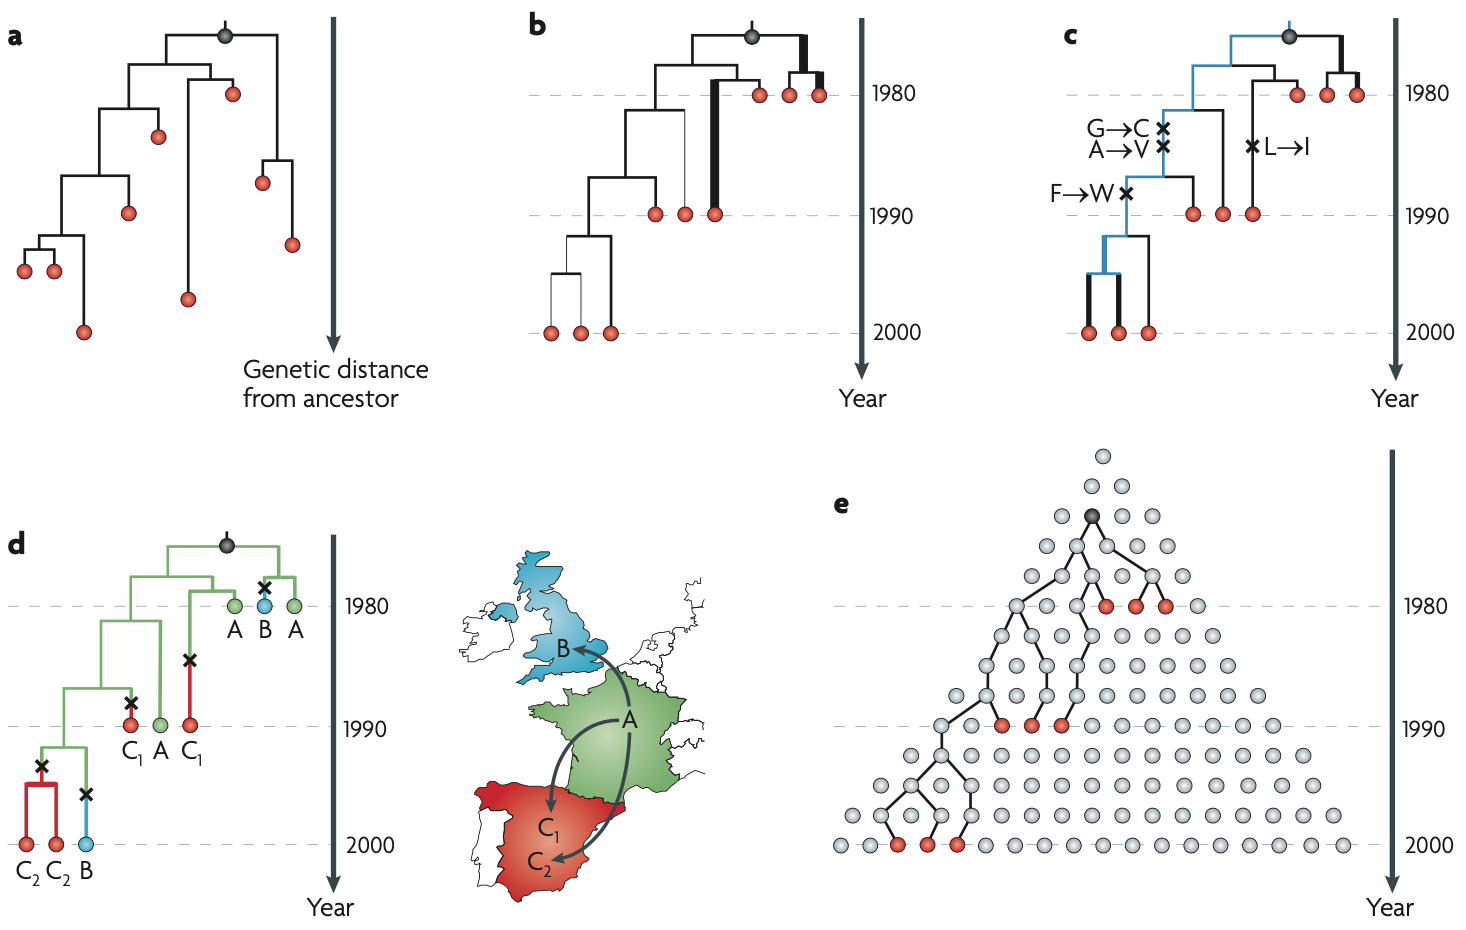
\includegraphics[width=.9\textwidth]{rambautFig}
  \caption[]{}
  \label{fig:phylogeneticsOverview}
\end{figure}

One particularly useful application of phylogenetics is in the analysis of viral pathogen outbreaks.
Viruses represent unique study systems for both the theoretical development of phylogenetic methodologies and the implementation of phylogenetic analyses in settings with tangible public health impact.
In addition to their ubiquity and high profile within the human population, viruses prove highly suitable for phylogenetic inference because of their fast evolutionary rates, small, simple genomes, and frequent adherence to the assumptions of a single evolutionary history (i.e. infrequent recombination or reassortment).
Phylogenetic methods have frequently been used to perform \textit{post hoc} analyses of viral outbreaks, however significant work is still required before such methods can be used to inform public health responses in ``real time" during an ongoing epidemic.
In this thesis, we describe phylogenetic analyses of three viral pathogens---Zika virus, Hepatitis B virus, and Lassa virus.
We use these analyses to both illustrate both the use of current phylogenetic analysis in performing retrospective analysis, and to provide a framework for so-called ``online" phylogenetic analyses that can be performed in real-time during a viral epidemic.

\section{Bayesian phylodynamics and joint inference}

In this thesis, we devote particular to Bayesian methodologies of phylogenetic inference.
Generally, Bayesian methods are those which do not assume that the parameters which govern statistical models take a single-point value, but rather come from some posterior probability distribution.
Such methodologies are also informed by hypotheses of these parameter distributions provided \textit{a priori} by researchers---referred to as parameter priors.
Bayesian methodologies are particularly well suited to phylogenetic methods in several key ways.
Firstly, they allow researchers to create robust estimates of evolutionary histories that still account uncertainty both in the phylogenies and in other parameters of interest.
Additionally, Bayesian phylogenetic methods afford researchers the opportunity to infer many different parameters of interest (e.g. mutation rates, effective population sizes, and migration rates) jointly with the phylogeny.
Finally, these methods can be put to use with relative ease using algorithms that allow efficient exploration of posterior distributions for many parameters simultaneously.

To perform Bayesian analyses it is frequently necessary to compute very large, highly dimensional integrals to produce exact posterior distributions; this is unfortunately often infeasible to solve analytically using computers.
However, this process can be made computationally tractable by defining a Markov Chain whose stationary distribution is the desired posterior distribution of parameters.
Through this implementation, we can use Markov Chain Monte Carlo (MCMC) methods to numerically solve for all desired parameter posterior distributions.

The implementation of such methods works according to a modified Metropolis-Hastings algorithm: first by creating a starting proposal for each parameter that is to be inferred by drawing from its prior distribution.
For numeric parameters this takes the form of one or more numbers being generated randomly, and a random tree topology is used as the initial tree.
A likelihood for the model can then be calculated, conditioned on the proposed tree and parameter set.
The candidate parameter set and tree will then be randomly permuted according to various transition kernels---referred to as ``operators"---and a new likelihood is calculated.
If the proposed parameter set yield a higher likelihood than the initial set, they are accepted as the new proposal set.
If they have a likelihood lower than the first proposal, they will be accepted with probability proportional to the ratio of their likelihoods.
This process is then repeated, until a stable parameter and tree set are found.
This stable set is considered to be the posterior distribution from which we would like to sample.
We continue to repeat the process, recording the state of the chain at regular intervals, until the posterior has been sufficiently explored.

\subsection{Measurably evolving populations and temporal signal}

While performing phylogenetic analyses, we are often interested in
\cite{shapiroscience}

\subsubsection{Temporal signal}



\subsection{Statistical and computational challenges} %GB: I would turn this into 'Statistical and computational challenges'; or perhaps leave it but make sure to explain that an important aspect to consider is acquiring sufficiently high ESS values for all relevant parameters

One of the major challenges of phylogenetic inference is the vast size of the state space of potentially inferred variables.
The size of so-called ``tree space"---the set of all possible phylogenetic trees for a given dataset---scales at the rate $\frac{(2n-3)!}{2^{n-1}(n-1)!}$.
This is far too large to exhaustively explore for the datasets that we are interested in; for a dataset consisting of only thirty taxa, the number of possible rooted, labeled phylogenies numbers over $10^{38}$\cite{felsenstein2003inferring}.
For the datasets that we explore in this thesis---ranging in size to 769 taxa---this number grows to vastly overshadow the number of atoms in the observable universe.
As such, exhaustively exploring this space is impossible, and traversing this space algorithmically can still take considerable time.

\subsection{Burnin and effective sample size}
Bayesian phylogenetic inference of large, complex datasets can take upwards of a month of constant compute time before a chain stabilizes and begins to explore the posterior distribution.
\begin{itemize}
  \item Burnin happens first
  \item Convergence happens when the chain reaches the posterior
  \item Mixing is how we conceptualize how quickly the posterior is being explored
  \item ESS is how we quantify how completely the posterior has been explored
\end{itemize}

\subsection{BEAST}

For the analyses described in this thesis, we make use of the software package Bayesian Evolutionary Analysis Sampling Trees 1.10 \cite{beast} (BEAST) in tandem with its associated utility programs (BEAUti, Tracer).
BEAST a flexible tool in which many Bayesian phylogenetic models---and their associated priors and transition kernels---have been implemented and optimized such that large datasets may be easily specified and run efficiently on a wide variety of compute resources.
This tool implements Bayesian phylogenetic inference via Markov Chain Monte Carlo


%%%%%%%%%%%%%%%%%%%%%%%%%%%%%%%%%%%%%%%%%%%%%%%%%%
% Keep the following \cleardoublepage at the end of this file,
% otherwise \includeonly includes empty pages.
\cleardoublepage

% vim: tw=70 nocindent expandtab foldmethod=marker foldmarker={{{}{,}{}}}
